%% ================================================================
%% # DBIS Databases Hand-in Template
%% 
%% Template for students to hand-in their databases exercise solutions.
%% 
%% [Databases and Information Systems Group](https://dbis.dmi.unibas.ch/)
%%
%% ## Usage
%% 
%% Fill in the required fields and write your submission
%%
%% ## Issues
%%
%% See dbisdbhandin.sty for further information.
%% ================================================================
\documentclass{article}
\usepackage{dbisdbhandin}
\usepackage[english]{babel}
%% ================================================================
%%
%% General Information
%%
%% ================================================================
%%
%% Add your information here
\course       {Databases}
\semester     {Autumn 2025}
\exerciseno   {1}
\studenta     {Aiysha Frutiger}
\studentb     {Jannick Seper}
\studentc     {Luis Tritschler}
%% Comment if you do the exercises alone


%% ================================================================
%%
%% Common Packages
%%
%% ================================================================
%%
%% Useful common packages for this course

%% Include pdfs into latex
\usepackage{pdfpages}
%% \includepdf[pages=1,pagecommand={\pagestyle{fancy}}]{filename}

%% Drawing everything, with lots of libraries
\usepackage{tikz}
%% A library providing ER prefabs
\usetikzlibrary{er}
\usetikzlibrary{positioning,arrows.meta}
%% ================================================================
%%
%% Custom Packages
%%
%% ================================================================
%%
%% Add custom packages below:
%%

% \usepackage{mypackage}

%% ================================================================
%%
%% Custom Commands
%%
%% ================================================================
%%
%% DRY: Use commands when you use something often or you'd like
%% to define it only once
%%

\newcommand*{\TikZ}{Ti\textit{k}Z}


\begin{document}
\printfront
\task{}
\begin{figure}[hbtp]
  \centering
  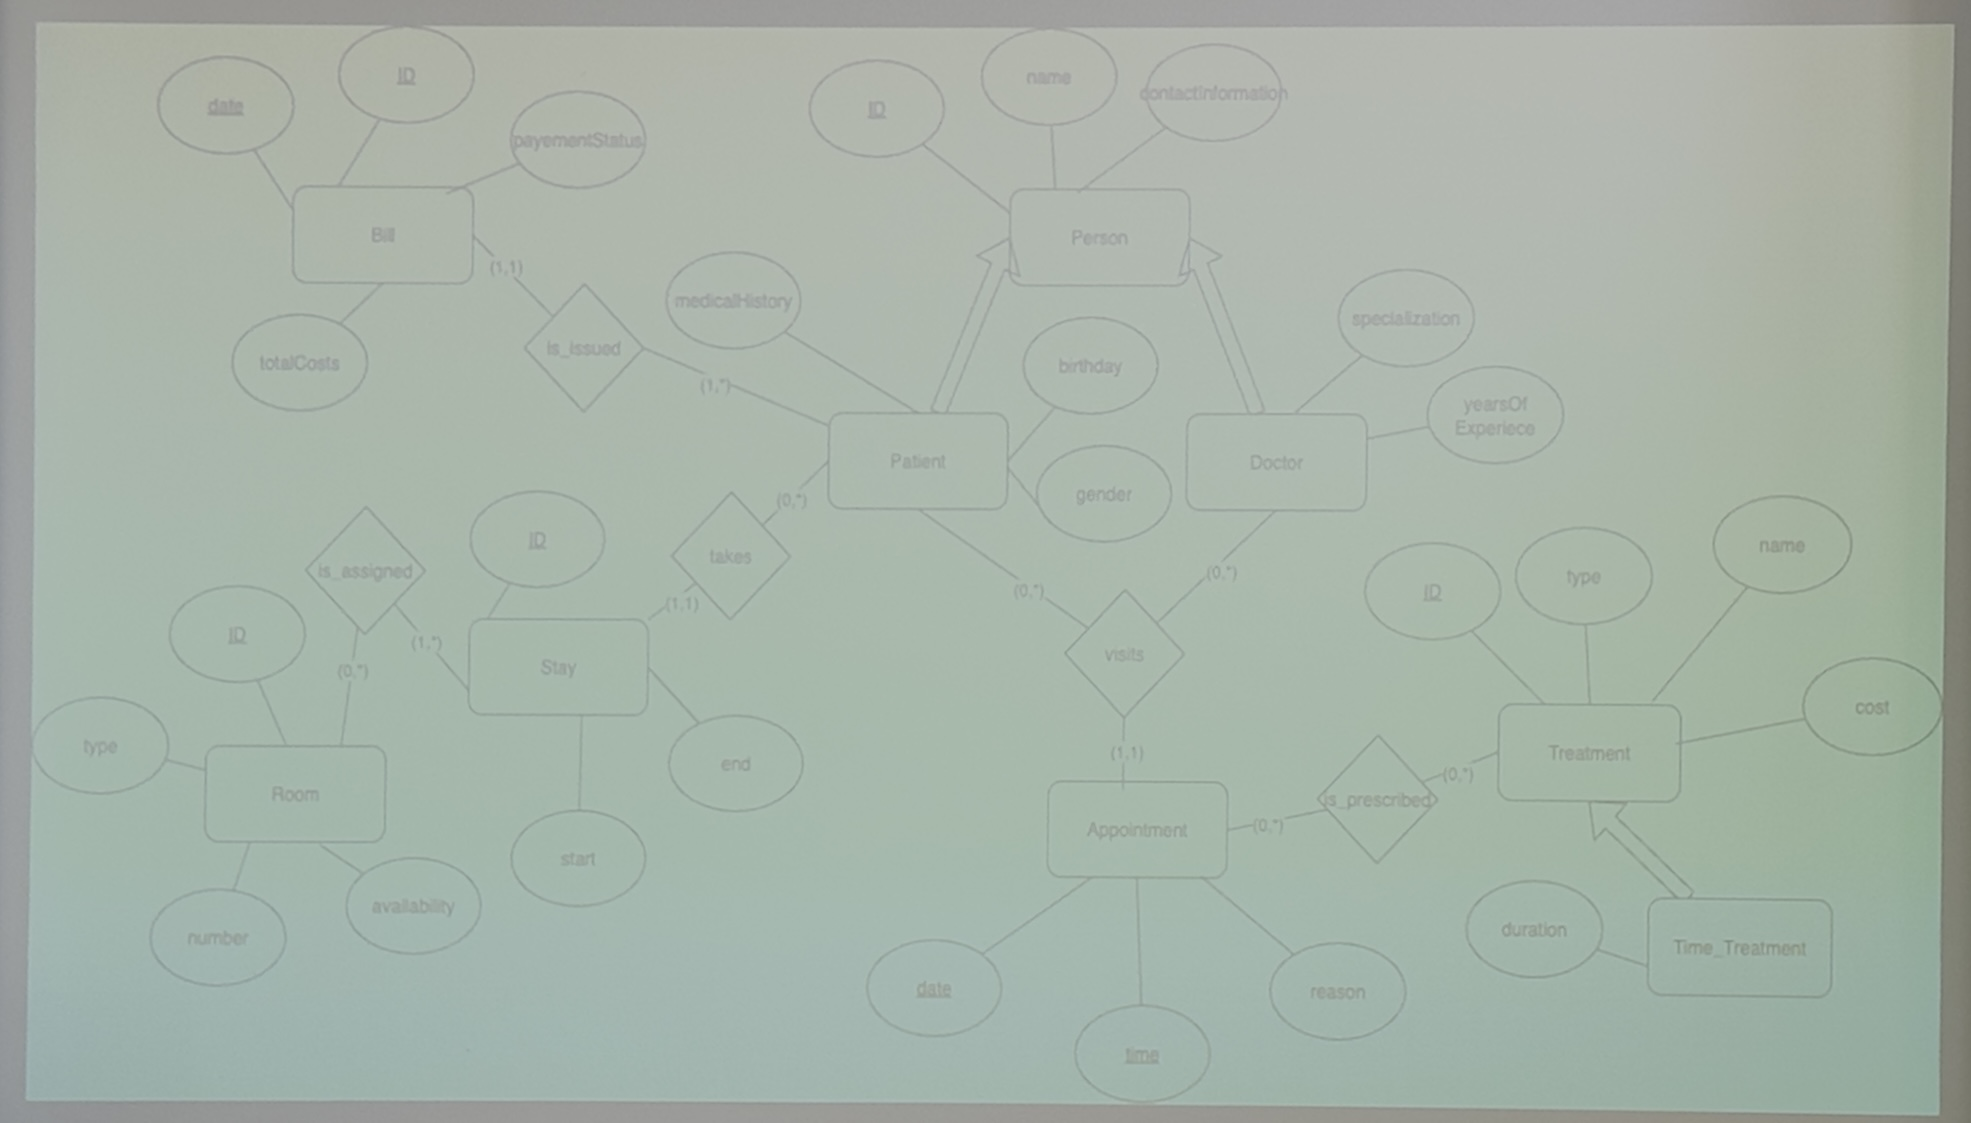
\includegraphics[width=\textwidth]{EER Model.jpeg} 
  \caption{EER}
  \label{fig:meinjpeg}
\end{figure}

\task{}
Out of the Picture:
\begin{center}
\begin{tabbing}
    Person \qquad\qquad\qquad\= (\uline{ID}, Name, ContactInformation)\\
    Doctor \> (\uline{ID}, Name, ContactInformation, Specialization, YearsOfExperience)\\
    Patient \> (\uline{ID}, Name, ContactInformation, Birthday, MedicalHistory, Gender)\\
    Appointment \> (\uline{Date, Time}, Reason)\\
    Stay \> (\uline{ID}, Start, End)\\
    Treatment \> (\uline{ID}, type, name, cost)\\
    Time\_Treatment \> (\uline{ID}, type, name, cost, duration)\\
    Bill \> (\uline{ID}, Date, TotalCosts, PaymentStatus)\\
    Room \> (\uline{ID}, Type, Number, Availability)\\[1em]
    visits \> (\uwave{Patient\_ID}, \uwave{Doctor\_ID}, \uwave{\uline{Date, Time}})\\
    takes \> (\uwave{\uline{Stay\_ID}}, \uwave{Patient\_ID})\\
    is\_prescribed \> (\uline{\uwave{Treatment\_ID}, \uwave{Date}, \uwave{Time}})\\
    is\_assigned \> (\uline{\uwave{Room\_ID}, \uwave{Stay\_ID}})\\
    is\_issued \> (\uwave{Patient\_ID}, \uline{\uwave{Bill\_ID}, \uwave{Date}})
\end{tabbing}
\end{center}

Merged:
\begin{center}
\begin{tabbing}
    Person \qquad\qquad\qquad\= (\uline{ID}, Name, ContactInformation, Birthday)\\
    Doctor \> (\uline{ID}, Name, ContactInformation, Birthday, Specialization, YearsOfExperience)\\
    Patient \> (\uline{ID}, Name, ContactInformation, Birthday, MedicalHistory)\\
    Appointment \> (\uline{Date, Time}, Reason, \uwave{Patient\_ID}, \uwave{Doctor\_ID})\\
    Stay \> (\uline{ID}, Start, End, \uwave{Patient\_ID})\\
    Treatment \> (\uline{ID}, type, name, cost)\\
    Time\_Treatment \> (\uline{ID}, type, name, cost, duration)\\
    Bill \> (\uline{ID}, Date, TotalCosts, PaymentStatus, \uwave{Patient\_ID})\\
    Room \> (\uline{ID}, Type, Number, Availability)\\[1em]
    is\_prescribed \> (\uline{\uwave{Treatment\_ID}, \uwave{Date}, \uwave{Time}})\\
    is\_assigned \> (\uline{\uwave{Room\_ID}, \uwave{Stay\_ID}})
\end{tabbing}
\end{center}


\task{}
Included SQL snippets to the questions:

\lstinputlisting[language=SQL,frame=single,numbers=left,numberstyle=\tiny]{SQL/a).sql}
\lstinputlisting[language=SQL,frame=single,numbers=left,numberstyle=\tiny]{SQL/b).sql}
\lstinputlisting[language=SQL,frame=single,numbers=left,numberstyle=\tiny]{SQL/c).sql}

\newpage
\task{}
Included SQL snippets to create DB (100\% ChatGPT):

\lstinputlisting[language=SQL,frame=single,numbers=left,numberstyle=\tiny]{SQL/4.sql}

\newpage
\task{}
Um das Schema auf einem MacBook mit PostgreSQL auszuführen, sind folgende Schritte nötig:

\begin{enumerate}
  \item \textbf{PostgreSQL installieren} (falls noch nicht vorhanden):\\

  \item \textbf{Neue Datenbank anlegen}:\\
  \begin{lstlisting}[language=bash]
  psql postgres
  \end{lstlisting}
  und im Prompt:
  \begin{lstlisting}[language=SQL]
  CREATE DATABASE hospital;         #creates DB
  \q                                #quits psql
  \end{lstlisting}

  \item \textbf{Schema-Datei ausführen}:\\
  \begin{lstlisting}[language=bash]
  cd /Pfad/zum/Ordner
  psql -d hospital -f schema.sql    #imports schema
  \end{lstlisting}

  \item \textbf{Tabellen testen}:\\
  \begin{lstlisting}[language=bash]
  psql hospital       
  \end{lstlisting}
  und im Prompt:
  \begin{lstlisting}[language=SQL]
  \dt             -- zeigt alle Tabellen
  \d appointment  -- zeigt Struktur von appointment
  \end{lstlisting}
\end{enumerate}

\end{document}
